\documentclass[11pt,a4paper]{article}

\usepackage[utf8]{inputenc}
\usepackage[T1]{fontenc}
\usepackage{lmodern}
\usepackage[margin=2.5cm]{geometry}
\usepackage{microtype}
\usepackage{booktabs}
\usepackage{tabularx}
\usepackage{enumitem}
\usepackage{xcolor}
\usepackage{tikz}
\usetikzlibrary{positioning,arrows.meta,fit,backgrounds,calc}
\usepackage[hidelinks]{hyperref}

\definecolor{accent}{HTML}{305496}
\definecolor{yescol}{HTML}{2E7D32}
\definecolor{nocol}{HTML}{C62828}
\newcommand{\yes}{\textcolor{yescol}{\textbf{Yes}}}
\newcommand{\no}{\textcolor{nocol}{\textbf{No}}}

\setlist{itemsep=2pt,topsep=4pt}

\title{\textbf{RPG Maker Superpowers}\\[4pt]
\large Vision: an extensible, modern editor for RPG Maker 2000/2003 games}
\author{Vision Document}
\date{7 October 2026}

\begin{document}
\maketitle

\begin{abstract}
RPG Maker 2000 and 2003 still have an active community, but both the editor and the
runtime are closed, Windows-only programs from the early 2000s. Existing patches add
fixed feature sets to the runtime or to the editor, yet no project lets users write
their own extensions for the \emph{editor itself}. This document describes a plan to
close that gap: a Godot-based editor for RPG Maker 2000/2003 projects, built on the
open-source EasyRPG ecosystem, in which every feature (new event commands, shader
support, pixel-perfect movement) can be added through a plugin system with an editor
half and a runtime half.
\end{abstract}

\tableofcontents

\section{Vision}

\textbf{Give RPG Maker superpowers.} Developers should be able to extend RPG Maker
2000/2003 in two directions:

\begin{enumerate}
  \item \textbf{The editor itself} -- new tools, new dialogs, new event commands with
        real user interfaces, live previews (for example shader previews in the map view).
  \item \textbf{The game} -- new mechanics such as pixel-perfect movement or shader
        support at runtime.
\end{enumerate}

The core idea is an \emph{extendable block}: a plugin system where users write code to
add functionality, instead of waiting for a single patch author to implement it.

\section{The existing landscape}

RPG Maker 2000/2003 has a long modding history. The most relevant projects are:

\begin{description}
  \item[Maniacs Patch] (BingShan) -- the de facto standard for RPG Maker 2003. Patches
        both editor and runtime with many new and extended event commands (string
        variables, extended variable operations, nested loops, mouse input, \ldots).
        Only works with the official Steam version of 2003. Actively developed, but
        closed source and not user-extensible; documentation is mostly in Japanese.
  \item[DynRPG] (Cherry) -- C++ plugin SDK for the 2003 runtime, source on GitHub.
        Plugins exist for OpenGL rendering with shaders and Lua scripting (RPGSS).
        Tied to runtime version 1.08; custom commands are written as event comments.
  \item[Destiny Patch] (Bananen-Joe) -- the RPG Maker 2000 counterpart, adding
        DestinyScript in event comments. Requires runtime version 1.07.
  \item[Ineluki's Key Patch] -- replaces \texttt{Harmony.dll}, the sound engine shared
        by 2000 and 2003, to run scripts.
  \item[EasyRPG Player] -- open-source (GPLv3, C++) reimplementation of the runtime for
        2000 and 2003, running on Windows, Linux, macOS, Android, consoles and the web.
        Prioritises compatibility with vanilla games and steadily implements Maniacs
        features, enabled only when a game uses them.
  \item[EasyRPG Editor] -- open-source (GPLv3, C++/Qt~6) editor that imports 2000/2003
        projects. Actively developed; its completeness (especially the event editor)
        still needs to be evaluated.
  \item[liblcf] -- EasyRPG's library for reading and writing 2000/2003 project and save
        files. Shared by Player and Editor.
\end{description}

\begin{table}[h]
\centering
\small
\begin{tabularx}{\textwidth}{@{}l c c l l c@{}}
\toprule
\textbf{Project} & \textbf{2000} & \textbf{2003} & \textbf{Constraint} & \textbf{Layer} & \textbf{User-extensible} \\
\midrule
Maniacs Patch       & \no  & \yes & Steam 2003 only   & Editor + runtime & \no \\
DynRPG              & \no  & \yes & Runtime v1.08     & Runtime          & \yes \\
Destiny Patch       & \yes & \no  & Runtime v1.07     & Runtime          & \yes \\
Ineluki's Key Patch & \yes & \yes & --                & Runtime          & Partly \\
EasyRPG Player      & \yes & \yes & --                & Runtime          & Open source \\
EasyRPG Editor      & \yes & \yes & Import            & Editor           & Open source \\
\bottomrule
\end{tabularx}
\caption{Existing projects at a glance.}
\end{table}

\subsection{The gap}

No project offers a \textbf{user-scriptable editor}. Maniacs changes the editor, but
only with its author's fixed feature set. DynRPG and Destiny extend the runtime only and
fall back to comment-based commands without editor support. On RPG Maker 2000 the gap
is even larger: there is no actively developed patch for the Steam version at all.

\section{Options considered}

\begin{enumerate}[label=\textbf{\Alph*.}]
  \item \textbf{Hook the vanilla editor.} A proxy DLL loaded into
        \texttt{RPG2000.exe}/\texttt{RPG2003.exe}, hooking the (presumably Delphi/VCL)
        user interface to add menus, dialogs and a Test Play redirect.
        \emph{Pros:} users keep the editor they know.
        \emph{Cons:} fragile reverse engineering against a moving target (Maniacs patches
        the same binaries), Windows-only, legally more delicate.
  \item \textbf{Extend EasyRPG Editor.} Add a plugin API to the existing Qt editor.
        \emph{Pros:} open source, shares liblcf with the Player.
        \emph{Cons:} depends on how complete the editor is today.
  \item \textbf{Godot as the editor, EasyRPG Player as the runtime.} \emph{Preferred direction.}
        A Godot editor plugin reads and writes the original project format via liblcf;
        games run in EasyRPG Player.
        \emph{Pros:} extensibility, shaders and a modern UI come with Godot; no reverse
        engineering; cross-platform.
        \emph{Cons:} the editor (especially the event editor) must be rebuilt.
  \item \textbf{Godot as editor \emph{and} runtime.} \emph{Rejected for now.} This
        would mean writing a new engine that exactly matches the behaviour of the
        original runtime -- the work EasyRPG has done over more than a decade.
\end{enumerate}

\noindent Option~C is the working direction. Before committing, the current state of
EasyRPG Editor (option~B) should be evaluated, since contributing to it may turn out to
be faster.

\section{Architecture}

\begin{figure}[h]
\centering
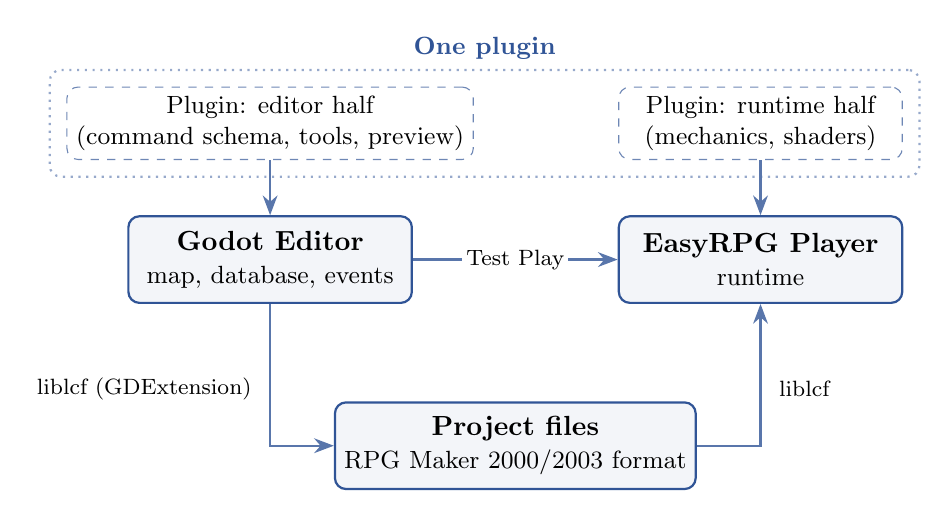
\begin{tikzpicture}[
  box/.style={draw=accent, thick, rounded corners, align=center, minimum width=3.6cm, minimum height=1.1cm, fill=accent!6},
  plug/.style={draw=accent!70, dashed, rounded corners, align=center, minimum width=3.6cm, minimum height=0.9cm, fill=white, font=\small},
  arr/.style={-{Stealth[length=2.5mm]}, thick, draw=accent!80},
  lbl/.style={font=\footnotesize, midway, fill=white, inner sep=1.5pt}
]
\node[box] (editor) {\textbf{Godot Editor}\\\small map, database, events};
\node[box, right=2.6cm of editor] (player) {\textbf{EasyRPG Player}\\\small runtime};
\node[box, below=1.8cm of $(editor)!0.5!(player)$] (files) {\textbf{Project files}\\\small RPG Maker 2000/2003 format};
\node[plug, above=0.7cm of editor] (ep) {Plugin: editor half\\(command schema, tools, preview)};
\node[plug, above=0.7cm of player] (rp) {Plugin: runtime half\\(mechanics, shaders)};

\draw[arr] (editor.south) |- node[font=\footnotesize, left=3pt, pos=0.3] {liblcf (GDExtension)} (files.west);
\draw[arr] (files.east) -| node[font=\footnotesize, right=3pt, pos=0.7] {liblcf} (player.south);
\draw[arr] (editor) -- node[lbl] {Test Play} (player);
\draw[arr] (ep) -- (editor);
\draw[arr] (rp) -- (player);

\begin{scope}[on background layer]
\node[draw=accent!50, dotted, thick, rounded corners, fit=(ep)(rp), inner sep=6pt,
      label={[font=\small\bfseries, text=accent]above:One plugin}] {};
\end{scope}
\end{tikzpicture}
\caption{Proposed architecture. Every feature ships as an editor half and a runtime
half; both sides meet in the original project file format.}
\end{figure}

\subsection{Components}

\begin{description}
  \item[liblcf as GDExtension] The complete data layer -- maps, database, events,
        command codes -- wrapped for Godot. This is the largest and most error-prone
        part of an editor, and it already exists.
  \item[Map view] Chipset and autotile rendering ported from (or modelled on) EasyRPG
        Player, whose implementation already matches the original exactly.
  \item[Data-driven event editor] Each event command is described by a schema
        (parameters, types, labels); Godot generates the dialog from it. This avoids
        hand-building over a hundred dialogs and is the foundation of the plugin system.
  \item[Plugin API] A plugin registers new command schemas, menus, docks and previews
        in the editor, and ships a matching runtime part for the Player.
  \item[Test Play] Launches EasyRPG Player as a separate process with the current
        project. Deeper embedding (for example via the libretro core) can come later.
  \item[Runtime extensions] Implemented in EasyRPG Player, ideally through an official
        plugin or scripting API developed together with the EasyRPG team rather than in
        a private fork.
\end{description}

\subsection{Storing new features}

New commands must be stored so that existing tools are not broken: initially as
structured event comments, later possibly using command codes the EasyRPG project
reserves for its own extensions. This has to be agreed with the EasyRPG team.

\section{Example extensions}

\begin{description}
  \item[Shader support] Editor half: a shader picker with live preview in the Godot
        map view. Runtime half: a GPU rendering path in EasyRPG Player. Note that the
        Player currently renders mostly on the CPU (SDL2/Pixman), so this is the larger
        of the two examples.
  \item[Pixel-perfect movement] Editor half: per-event settings such as hitboxes and
        movement speed in sub-tile units. Runtime half: replacement movement and
        collision logic in the Player.
\end{description}

\section{Design principles}

\begin{enumerate}
  \item \textbf{Opt-in.} New features are only active when a game uses them -- the same
        approach EasyRPG uses for Maniacs features.
  \item \textbf{Vanilla compatibility.} Vanilla, Maniacs and extended games all run on
        the same Player.
  \item \textbf{Original format first.} Projects stay in the RPG Maker 2000/2003 format,
        so they remain usable with existing tools wherever possible.
  \item \textbf{Cooperation over forking.} Work with the EasyRPG team and, where useful,
        contribute missing Maniacs features upstream.
  \item \textbf{No modified vendor binaries.} The project never patches or redistributes
        the original RPG Maker executables.
\end{enumerate}

\section{Licensing and legal notes}

\begin{itemize}
  \item EasyRPG Player and EasyRPG Editor are licensed under GPLv3. Code copied from
        them makes the Godot plugin GPLv3 as well -- acceptable for an open-source
        tool, and games made with the editor are not affected as long as the plugin's
        code does not end up inside them.
  \item liblcf uses the permissive MIT license (confirmed in its COPYING file), so a
        Godot extension built only on liblcf can use any license. This project starts
        as MIT and would move to GPLv3 only if EasyRPG code is ported into it.
  \item If the vanilla editor is ever analysed (option~A), §69e UrhG permits
        decompilation in limited cases for interoperability. Distribution should always
        take the form of a separate loader, never modified executables.
  \item These notes are not legal advice.
\end{itemize}

\section{Risks and open questions}

\begin{itemize}
  \item How complete is EasyRPG Editor today? Does it save back to the original format,
        so the vanilla editor can still open projects?
  \item Is the EasyRPG team open to a plugin or scripting API in the Player (and Editor)?
  \item Scope of the event editor, even with data-driven dialogs.
  \item Shader support requires a GPU renderer in the Player.
  \item Adoption: many 2003 developers rely on Maniacs and its editor.
\end{itemize}

\section{Roadmap}

\begin{enumerate}[label=\textbf{M\arabic*}, start=0]
  \item \textbf{Evaluate and connect.} Test an EasyRPG Editor daily build on a real
        project (including a save round trip). Contact the EasyRPG team about the vision
        and a plugin API.
  \item \textbf{liblcf in Godot.} GDExtension that loads a 2000/2003 project.
  \item \textbf{Map view.} Display one map with correct chipsets and autotiles.
  \item \textbf{Database viewer.} Browse and edit database entries.
  \item \textbf{Event editor.} Schema-driven dialogs for the built-in commands.
  \item \textbf{Plugin API (editor).} Plugins register commands, menus and docks.
  \item \textbf{Test Play and runtime half.} Launch EasyRPG Player; first runtime
        extension mechanism.
  \item \textbf{Showcase plugins.} Pixel-perfect movement, then shader support.
\end{enumerate}

\section*{References}
\addcontentsline{toc}{section}{References}

\begin{itemize}
  \item EasyRPG Player: \url{https://github.com/EasyRPG/Player}
  \item EasyRPG Editor: \url{https://github.com/EasyRPG/Editor}
  \item liblcf: \url{https://github.com/EasyRPG/liblcf}
  \item EasyRPG documentation: \url{https://wiki.easyrpg.org}
  \item Maniacs support tracking issue: \url{https://github.com/EasyRPG/Player/issues/1818}
  \item Maniacs Patch: \url{https://bingshan1024.github.io/steam2003_maniacs/}
  \item DynRPG source: \url{https://github.com/CherryDT/DynRPG}
  \item RMteka Maniacs article series: \href{https://www.rmteka.pl/maniacs-patch-wont-bite-you-1-basic-feature-changes/}{rmteka.pl, ``Maniacs Patch Won't Bite You'' series}
\end{itemize}

\end{document}
